\documentclass[conference]{IEEEtran}

\usepackage{booktabs} % For formal tables
\usepackage{listings}
\usepackage{url}
\usepackage{color}
%\usepackage{authblk}
\usepackage{graphicx}
\usepackage{subcaption}
\captionsetup{compatibility=false}


%\renewcommand{\baselinestretch}{0.945}
%\newcommand*\samethanks[1][\value{footnote}]{\footnotemark[#1]}

% Copyright
%\setcopyright{none}
% \setcopyright{acmcopyright}
%\setcopyright{acmlicensed}
% \setcopyright{rightsretained}
%\setcopyright{usgov}
%\setcopyright{usgovmixed}
%\setcopyright{cagov}
%\setcopyright{cagovmixed}


% DOI
% \acmDOI{10.475/123_4}

% ISBN
% \acmISBN{123-4567-24-567/08/06}

%\acmPrice{15.00}


\begin{document}


\newcommand{\mike}[1]{\textcolor{red}{#1}}
\newcommand{\vaibhav}[1]{\textcolor{red}{#1}}
\newcommand{\soha}[1]{\textcolor{red}{#1}}
\newcommand{\smcc}[1]{\textcolor{red}{#1}}

\newcommand{\toolshort}{JR}
\newcommand{\tool}{Java Ranger}
\newcommand{\toolfull}{Java Ranger}

\title{\tool: Static Regions for Efficient Symbolic Execution of Java}
%\author{\IEEEauthorblockN{Vaibhav Sharma}
%\IEEEauthorblockA{Department of Computer Science and\\Engineering\\
%University of Minnesota\\
%Minneapolis, MN 55455\\
%vaibhav@umn.edu}
%\and
%\IEEEauthorblockN{Soha Hussein}
%\IEEEauthorblockA{Department of Computer Science and\\Engineering\\
%University of Minnesota\\
%Minneapolis, MN 55455\\
%husse200@umn.edu}
%\and
%\IEEEauthorblockN{Michael W. Whalen}
%\IEEEauthorblockA{Amazon Web Services\\
%mww@amazon.com}
%\and
%\IEEEauthorblockN{Stephen McCamant}
%\IEEEauthorblockA{Department of Computer Science and\\Engineering\\
%University of Minnesota\\
%Minneapolis, MN 55455\\
%mccamant@cs.umn.edu}
%\and
%\IEEEauthorblockN{Willem Visser}
%\IEEEauthorblockA{Computer Science Division\\
%University of Stellenbosch\\
%Stellenbosch, South Africa\\
%wvisser@cs.sun.ac.za}
%}

%\author{
%\IEEEauthorblockN{{\bf Vaibhav Sharma}\IEEEauthorrefmark{1}\\ \tt\footnotesize vaibhav@umn.edu} \and
%\IEEEauthorblockN{{\bf Soha Hussein}\IEEEauthorrefmark{1}\\ \tt\footnotesize husse200@umn.edu} \and
%\IEEEauthorblockN{{\bf Michael W. Whalen}\IEEEauthorrefmark{2}\\ \tt\footnotesize mww@amazon.com} \and
%\IEEEauthorblockN{{\bf Stephen McCamant}\IEEEauthorrefmark{1}\\ \tt\footnotesize mccamant@cs.umn.edu} \and
%\IEEEauthorblockN{{\bf Willem Visser}\IEEEauthorrefmark{3}\\ \tt\footnotesize wvisser@cs.sun.ac.za} \and
%\IEEEauthorblockA{\IEEEauthorrefmark{1}Department of Computer Science and Engineering,  University of Minnesota, Minneapolis, MN 55455}
%\IEEEauthorblockA{\IEEEauthorrefmark{2}Amazon Web Services}
%\IEEEauthorblockA{\IEEEauthorrefmark{3}University of Stellenbosch, Stellenbosch, South Africa}
%}

\author{\IEEEauthorblockN{Vaibhav Sharma\IEEEauthorrefmark{1},
Soha Hussein\IEEEauthorrefmark{1},
Michael W. Whalen\IEEEauthorrefmark{2},
Stephen McCamant\IEEEauthorrefmark{1} and
Willem Visser\IEEEauthorrefmark{3}}
\IEEEauthorblockA{\IEEEauthorrefmark{1}Department of Computer Science and Engineering,  University of Minnesota, Minneapolis, MN 55455\\
Email: \{vaibhav, husse200, smccaman\}@umn.edu}
\IEEEauthorblockA{\IEEEauthorrefmark{2}Amazon Web Services,\\
Email: mww@amazon.com}
\IEEEauthorblockA{\IEEEauthorrefmark{3}Computer Science Division,
University of Stellenbosch,
Stellenbosch, South Africa,\\
Email: wvisser@cs.sun.ac.za}
}

\maketitle
\begin{abstract}

%Scaling symbolic execution to industrial-sized programs is an important open research problem.  Veritesting introduced bounded static regions in symbolic execution to improve scalability by combining the advantages of static symbolic execution with those of dynamic symbolic execution.  Bounded static regions reduce the number of paths to explore in symbolic execution by describing regions of code using disjunctive formulas.
%%
%In previous work, veritesting was applied to binary-level symbolic execution.

%Integrating veritesting with Java bytecode presents unique challenges, 
%notably, incorporating many more non-local control jumps caused by runtime polymorphism, exceptions, native calls, and dynamic class loading.
%%
%If these languages features are not accounted for, the static code regions described by veritesting are often small and may not lead to substantial reduction in paths.  In addition, the use of disjunctive regions forces previously concrete assignments to become symbolic leading to additional solver calls.  

%In this paper, we describe \tool, which adds static regions to Java Symbolic Pathfinder.  Unlike previous approaches, it adds support for {\em higher order} Veritesting regions into which we can instantiate static regions for staticly- and dynamically-dispatched function calls.  Although our tool is still an unoptimized prototype, we show that it dramatically outperforms Java Symbolic Pathfinder on a number of benchmark examples, and that support for higher-order regions substantially improves the performance of Veritesting for Java programs.

Merging related execution paths is a powerful technique for reducing
path explosion in symbolic execution.
%
One approach, introduced and dubbed ``veritesting'' by Avgerinos et
al., works by statically translating a bounded control flow region
into a single formula.
%
This approach is a convenient way to achieve path merging as a
modification to a pre-existing single-path symbolic execution engine.
%
Avgerinos et al. evaluated their approach in a symbolic execution tool
for binary code, but different design considerations apply when
building tools for other languages.
%
In this paper we explore the best way to use a veritesting approach in
the symbolic execution of Java.

Because Java code typically contains many small dynamically dispatched
methods, it is important to include them in veritesting regions; we
introduce a {\em higher-order} veritesting technique to do so
modularly.
%
Java's typed memory structure is very different from a binary, but we
show how the idea of static single assignment (SSA) form can be
applied to object references to statically account for aliasing.
%
More formally, we describe our veritesting algorithms as
syntax-directed transformations of a structured intermediate
representation, which highlights their logical structure.
%
We have implemented our algorithms in \tool, an extension to the
widely used Symbolic Pathfinder tool for Java bytecode.
%
Our empirical evaluation shows that veritesting greatly reduces the
search space of Java symbolic execution benchmarks, while our expanded
capabilities provided a significant further improvement.



\end{abstract}

%\keywords{multi-path symbolic execution; veritesting; Symbolic
%PathFinder; static analysis}


%Path explosion problem is still the main obsticale against scaling up symbolic execution to industrial sized projects.
%%
%One interesting resolution to the problem is \emph{Veritesting}, which represents regions of code as disjunctive formals over paths.
%%
%Unlike the C compiler that inlines functions in programs, Integrating veritesting with Java bytecode presents unique challenges: notably, incorporating non-local control jumps caused by runtime polymorphism, exceptions, native calls, and dynamic 3 class loading.
%%
%In this paper we present our robust implementation of Java based veritesting tool that supports dynamic dispatch and
\section{Introduction}
\vaibhav{needs rewriting, assigned to anyone who can find the time to write it}

Symbolic execution is a popular analysis technique that performs non-standard execution of a program: data operations generate formulas over inputs, and the branch constrains along an execution path are combined into a predicate.
%
Originally developed in the 1970s~\cite{King1976,Clarke1976}, symbolic execution is a convenient building block for program analysis, since arbitrary query predicates can be combined with the logical program representation, and solutions to these constraints are program inputs illustrating the queried behavior.
%
Some of the many application of symbolic execution include
test generation~\cite{dart,cute}, equivalence checking~\cite{ramos,adaptorsynth}, vulnerability finding~\cite{driller,angr}, and protocol correctness checking~\cite{transport}.
%
Symbolic execution tools are available for many languages, including
CREST~\cite{BurnimS2008} for C source code, KLEE~\cite{CadarDE2008}
for C/C++ via LLVM, JDart~\cite{jdart2016} and Symbolic
PathFinder~\cite{spf} for Java, and S2E~\cite{ChipounovKC2012},
FuzzBALL~\cite{BabicMMS2011}, and angr~\cite{angr} for binary code.
%
 \mike{More here...explain the `ecosystem' - tools for different languages: KLEE, FuzzBall, Java Symbolic Pathfinder, ...}

Although symbolic analysis is a very popular technique, scalability is a substantial challenge for symbolic execution.
%
Dynamic state merging~\cite{kuznetsov} provides one way to
alleviate scalability challenges by opportunistically merging dynamic
symbolic executors, which can be performed on paths~\mike{Add std. cite} or on environments~\mike{FM paper from 2014 on Javascript?}.  
Other techniques include CEGAR/subsumption~\mike{Add references from ASE 2017 paper: More Effective Interpolations in Software Model Checking}.
 
%
Veritesting~\cite{veritesting} is a different recently proposed technique that can dramatically improve the performance of symbolic execution.  Rather than explicitly merge paths or check subsumption relationships, Veritesting simply encodes a local region of a program containing branches as a disjunctive region for symbolic analysis.  If any path within the region meets an exit point, then the disjunctive formula is satisfiable.  This often allows many paths to be collapsed into a single path involving the region.  
%
In previous work~\cite{veritesting}, bounded static code regions have been shown to find more bugs, and achieve more node and path coverage, when implemented at the X86 binary level for compiled C programs.
%
This provides motivation for investigating integration of introducing static regions with symbolic execution at the Java bytecode level.

\lstinputlisting[caption={An example to loop through a symbolic array with three execution paths through the loop body},
label={lst:v_ex}]{code_samples/VeritestingPerf.java}



%Symbolic Pathfinder~(SPF)~\cite{spf} is a tool that performs symbolic execution of Java bytecode.
%
%SPF is tightly integrated with Java PathFinder~(JPF)~\cite{jpf} and uses JPF extensions to replace concrete execution with symbolic execution.
%
We present an example demonstrating the potential benefit of integrating static code regions with SPF in Listing~\ref{lst:v_ex}.
%
The example checks if positive or negative integers occur more frequently in the
list~\textit{x}, and it contains a bug if \textit{x} contains an
equal number of positive and negative integers.
%
The three-way branch on lines 5, 6 causes the total number of execution
paths required to cover the \textit{for} loop to be $3^{\textit{len}}$.
%
However, this three-way branch can be combined into a multi-path region
and represented as a disjunctive predicate.
We present such predicates in SMT2 notation in
Listing~\ref{lst:v_ex_smt2} assuming \textit{x} to contain two symbolic
integers named \textit{x0} and \textit{x1}~(\textit{len} equals 2).
%
The updates to \textit{sum} in the two loop iterations are captured by
\textit{sum0} and \textit{sum1}.
%
Using such predicates to represent the three-way branch on lines 5, 6 of
Listing~\ref{lst:v_ex} allows us to have only one execution path through
the loop body.
%
Figure~\ref{fig:v_ex_plot} shows a comparison of the number of execution
paths explored to find the bug on line 11 of Listing~\ref{lst:v_ex}.
%
The exponential speed-up from our predicates, representing a multi-path
region, allows us to find
the bug using just three test cases.

Unfortunately, as originally proposed, Veritesting would be unable to create a static region for this loop because it involves non-local control jumps (the calls to the \texttt{get} methods).  This is not an impediment for compiled C code, as the C compiler will usually automatically inline the code for short methods such as \texttt{get}.  However, Java has an {\em open world} assumption, and most methods are {\em dynamically dispatched}, meaning that the code to be run is not certain until resolved at runtime, so the compiler is unable to perform these optimizations.

In Java, programs often consist of many small methods that are dynamically dispatched, leading to poor performance for n\"aive implementations of bounded static regions.  Thus, to be successful, we must be able to inject the static regions associated with the calls into the dispatching region.  We call such regions {\em higher order} as they require a region as an argument and can return a region that may need to be further interpreted.
Given support for such regions, we can make analysis of programs such as~\ref{lst:v_ex} trivial for large loop depths.  In our experiments, we demonstrate 100x speedups on several models (in general, the more paths contained within a program, the larger the speedup) over the unmodified Java SPF tool using this approach.
 
%
\lstinputlisting[caption={SMT2 representation of multi-path execution in
Listing ~\ref{lst:v_ex} using \textit{len} = 2}, label={lst:v_ex_smt2}, language=lisp]{code_samples/ex.smt2.snippet}
%
\begin{figure}[]
\caption{Comparing number of execution paths from Listing~\ref{lst:v_ex} using vanilla SPF and SPF with static unrolling}
\label{fig:v_ex_plot}
\includegraphics[width=\columnwidth]{figures/veritesting_example_semilogy}
\end{figure}
%
\subsection{Motivating Example}
\vaibhav{assigned to Vaibhav}

%\section{Preliminaries}
\subsection{CFG}
A control flow graph (CFG) in computer science is a representation, using graph notation, of all paths that might be traversed through a program during its execution.
In a control flow graph each node in the graph represents a basic block, i.e. a straight-line piece of code without any jumps or jump targets; jump targets start a block, and jumps end a block. Directed edges are used to represent jumps in the control flow. There are, in most presentations, two specially designated blocks: the entry block, through which control enters into the flow graph, and the exit block, through which all control flow leaves.

\subsection{SPF}
Symbolic PathFinder (SPF) \cite{spf} combines symbolic execution with model checking and constraint solving for test case generation. In this tool, programs are executed on symbolic inputs representing multiple concrete inputs. Values of variables are represented as numeric constraints, generated from analysis of the code structure. These constraints are then solved to generate test inputs guaranteed to reach that part of code. Essentially SPF performs symbolic execution for Java programs at the bytecode level. Symbolic PathFinder uses the analysis engine of the Ames JPF model checking tool (i.e. jpf-core) \cite{jpf}.


\subsection{Veritesting}
Veritesting\cite{veritesting} is a technique that reduces the number of paths that need to be explored by avoiding unnecessary forking. 
%
Veritesting identifies regions of if-statements that can be statically explored and captured in a logical formula (usually as disjunction of formulas representing different branches in if-statement). 
%
We will call this formula VeriFormula which captures possible different execution paths. 
%
The result of this process is a VeriFormula, which can be submitted to a SMT solver. 
%
If the formula is satisfiable, then there is some path through the code region that reaches the exit point. In this case, dynamic symbolic execution is resumed after updating the PC with the VeriFormula and also updating symbolic values of variable if needed. 

%\section{Challenges}

While the performance improvement demonstrated on the code in Listing 1 is impressive, it is perhaps not representative of most Java code.  Java conventions encourage the use of indirection when accessing class fields using non-static {\em get} and {\em set} methods, as well as liberal use of exceptions.  Unlike C compilers, which assume a ``closed world'' and often inline simple functions into the body of calling methods to improve performance, the Java compiler must assume an ``open world'' in which a class may be used in a new context, so inlining of non-final methods is unsafe.

Previous approaches to veritesting exit static code regions when indirect calls to functions or non-local jumps are made.  In this section, we explore how the structure of Java programs reducees the performance of a n\"aive veritesting approach.

%Talk about how veritesting is different when done on Java bytecode
%
%The transition points at the Java bytecode level are return, exceptions (done using athrow), virtual function invocations (invokevirtual, invokeinterface), native calls (also done using invokevirtual), reflection and dynamic class loading (also done using invokevirtual).
%
%Present results from Soot-based static analysis
%
%Talk about how veritesting gets harder to do when considering multi-threaded Java bytecode.
\subsection{Exit Points}
\label{sec:exit_points}

\mike{Should we re-run this analysis with WALA for consistency's sake?}
%While the performance improvement shown in Figure~\ref{fig:v_ex_plot} with statically unrolling the three-way branches is clear, we need to automate this process.
%
Integrating veritesting with SPF requires that we can represent a region of a Java program as a disjunctive formula with multiple exit points.  Each exit point describes a possible distinct continuation of the current path after the static code region completes execution.  Avgerinos et al.~\cite{veritesting} defined exit points as unresolved jumps, function boundaries, and system calls.
%
These exit points are nodes in a control-flow graph which represent non-local control flow, and therefore, need to be explored using plain dynamic symbolic execution.
%
In the context of Java bytecode, we find such non-local control flow in five ways listed as follows: (1) return statements, (2) exceptions, (3) virtual function invocations~(\textit{invokevirtual}, \textit{invokeinterface}), (4) reflection, (5) native calls.
%
\iffalse
\mike{These explanations are obvious and can be dispensed with if we need space}
Return statements form the function boundary, and are obvious candidates to be considered as exit points.
%
Exceptions are used to catch unexpected behavior, and often help design of cleaner code, and allow developers to capture useful information when such errors occur.
%
Virtual function invocations occur due to runtime polymorphism supported by Java.
%
The runtime environment binds the method call to its body by using the type of the object making the call.
%
Using reflection requires loading a class at runtime, identifying a method within the class, and calling it.
%
It is primarily used for extensibility purposes, achieving separate compilation, and generating a class at runtime.
\fi
%
%An approach such as Avgerinos et al.~\cite{veritesting} would force
%static code regions when any of these five constructs are encountered.

%Such regions must correctly preserve the semantics of symbolic execution for all possible Java constructs.
%
The primary benefit of implementing veritesting comes from its conversion of branches into disjunctions in a multi-path region.
%
But this benefit exists only when the number of different exit points from the disjunctive formula is less than the number of execution paths through the region in the first place.
%
For example, all execution paths in the first three-way branch in
Listing~\ref{lst:v_ex} joined together on line 7, causing the three-way branch to have a single exit point.
%
Therefore, it is crucial for us to study the number of exit points for each of our statically-analyzed regions vs. the number of branches within the region.
%
%
%Native calls are used to execute code outside of the Java Runtime Environment.
%
%Incorporating these into our static analysis would require handling virtual function invocations as well as static analysis of binary code.

These five types of exit points create the kind of non-local control flow which formed the frontier of the visible control-flow graph created as a result of \textit{CFGReduce} step by Avgerinos et al.
%
However, many of these exit points are used pervasively by Java developers.
%
For example, the Visitor design pattern is used extensively by the ASM framework~\cite{asm}, Soot~\cite{soot} and makes use of Java\rq s dynamic dispatch mechanism.
%
Running into exit points too often causes our statically-analyzed regions to be small and our performance gain from having fewer branches to be lost.

We investigated the occurrence of these exit points by creating a Soot-based static analysis of six large open-source projects written in Java.
%
Software faults from these six projects are maintained in the Defects4J~\cite{defects4j} repository.
%
We used Soot to create a control-flow graph for every method body in every class file in these six projects.
%
For each control-flow graph, we used nodes corresponding to conditional jump bytecodes as a starting point of our analysis.
%
We measured the number of instructions encountered when traversing down each side of the branch until we get to the immediate post dominator~\cite{dragon-book} of our starting point.
%
If there were no exit points encountered on any side of the branch, we considered this region as a pure multi-path region and calculated its size in bytecode instructions.
%
Finally, we allowed up to five nested branches and calculated the number of bytecode instructions from the earliest, as well as, the latest starting point in our control-flow graph traversal to an exit point.

As an example, we modify the three-way branch in Listing~\ref{lst:v_ex} by adding a {\tt else return;} to get the snippet shown in Listing~\ref{lst:v_ex_modified}.
%
\lstinputlisting[caption={Listing~\ref{lst:v_ex} modified to have a return statement in the three-way branch},
label={lst:v_ex_modified}, language=Java]{code_samples/VeritestingPerf_modified.java}
%
This results in bytecode that produces the control-flow graph shown in Figure~\ref{fig:v_ex_cfg}.
%
Nodes are numbered 1 through 6 with node (1) being the starting point and node (6) being the immediate post-dominator of node (1).
%
Nodes contain bytecode instructions along with instruction offsets.
%
The added \textit{return} statement creates an exit point, which causes the three-way branch in Listing~\ref{lst:v_ex_modified} to contain two exit points.
%
Counting the number of instructions after the {\tt ifge} instruction in node (1) through node (2) to node (6) gives us two instructions.
%
The same count going through nodes (3) and (4) to (6) gives us 6 instructions, and through nodes (3) to (5) gives us 4 instructions.
%
The presence of the \textit{return} statement in node (5) prevents this region from being a pure multi-path region.
%
\begin{figure}[]
\caption{Control-flow graph with {\tt else return;} added as line 7 of Listing~\ref{lst:v_ex}}
\label{fig:v_ex_cfg}
\includegraphics[width=\columnwidth]{figures/v_ex_cfg}
\end{figure}

%
We report our results from a Soot-based static analysis in Tables~\ref{t:r_s} and~\ref{t:r_c}.
%
\begin{table}[]
\centering
\begin{tabular}{|l|l|l|l|l|l|}
\hline
        & \#classes & \begin{tabular}[c]{@{}l@{}}if-\\ return\end{tabular} & \begin{tabular}[c]{@{}l@{}}if-\\ invokevirtual\end{tabular} & \begin{tabular}[c]{@{}l@{}}if-\\ throw\end{tabular} & \begin{tabular}[c]{@{}l@{}}region \\ size\end{tabular} \\ \hline
chart   & 679       & 8.44                                                 & 27.47                                                       & 4.33                                                & 13.59                                                  \\ \hline
closure & 1339      & 7.35                                                 & 22.1                                                        & 9.5                                                 & 11.66                                                  \\ \hline
lang    & 170       & 6.70                                                 & 11.64                                                       & 7.09                                                & 9.60                                                   \\ \hline
math    & 1104      & 18.27                                                & 56.61                                                       & 9.56                                                & 27.06                                                  \\ \hline
mockito & 382       & 6.02                                                 & 12.51                                                       & 8.05                                                & 13.57                                                  \\ \hline
time    & 209       & 7.79                                                 & 13.10                                                       & 7.08                                                & 8.10                                                   \\ \hline
\end{tabular}
\caption{Soot-based analysis for number of bytecode instructions between starting and exit points}
\vspace{-0.3in}
\label{t:r_s}
\end{table}
%
%\vspace{-0.7in}
%
\begin{table}[]
\centering
\begin{tabular}{|l|l|l|l|l|}
\hline
        & \begin{tabular}[c]{@{}l@{}}if-\\ return\end{tabular} & \begin{tabular}[c]{@{}l@{}}if-\\ invokevirtual\end{tabular} & \begin{tabular}[c]{@{}l@{}}if-\\ throw\end{tabular} & \begin{tabular}[c]{@{}l@{}}region\\ count\end{tabular} \\ \hline
chart   & 1712                                                 & 7760                                                        & 521                                                 & 6627                                                   \\ \hline
closure & 3853                                                 & 7466                                                        & 138                                                 & 9258                                                   \\ \hline
lang    & 3602                                                 & 1589                                                        & 539                                                 & 2065                                                   \\ \hline
math    & 2219                                                 & 5582                                                        & 662                                                 & 15375                                                  \\ \hline
mockito & 372                                                  & 572                                                         & 15                                                  & 574                                                    \\ \hline
time    & 1202                                                 & 984                                                         & 204                                                 & 1421                                                   \\ \hline
\end{tabular}
\caption{Number of occurences in Soot-based static analysis}
\vspace{-0.2in}
\label{t:r_c}
\end{table}
%
Table~\ref{t:r_s} shows the average size and Table~\ref{t:r_c} shows the number of times each such count was reported.
%\mike{We need to explain these tables better: can we take a small code fragment (say, that of Listing 1) and explain it according to these numbers, or create a very tiny code fragment that demonstrates them?}
%
The \textit{if-return}, \textit{if-invokevirtual}, \textit{if-throw} columns in Table~\ref{t:r_s} report the average number of instructions observed between any \textit{if} opcode-containing bytecode instruction and a \textit{return}, \textit{invokevirtual} or \textit{invokeinterface}, \textit{throw} opcode-containing bytecode instruction.
%
These same columns in Table~\ref{t:r_c} report the number of times we observed an occurence of one of \textit{return}, \textit{invokevirtual}, \textit{invokeinterface}, \textit{throw} opcode-containing bytecode instructions before reaching the immediate post-dominator of the starting \textit{if} node on any side of the branch.
%
Tables~\ref{t:r_s} and~\ref{t:r_c} show that while we discover thousands of regions which do not contain any exit points, these regions are small.
%
They also show that early \textit{return} instructions are another often used construct in Java.
%
We believe that creating multi-path regions for these no-exit-point cases alone would provide a significant performance boost to SPF.
%
Table~\ref{t:r_c} shows \textit{invokevirtual} or \textit{invokeinterface} instructions are encountered far more often than \textit{return} or \textit{throw} instructions.
%
This can be explained by the pervasive use of runtime polymorphism and exception handling by Java developers.
%
Instead of using \textit{invokevirtual} and \textit{invokeinterface}
instructions as exit points, if we can continue our predicate
construction for multi-path regions beyond them, we would almost double
the number of multi-path regions.
%

\iffalse
\subsection{Engineering Challenges}
Research challenges such as static analysis of exit points and veritesting in a multi-threaded context need to be solved for integrating veritesting with any bytecode-level symbolic execution engine.
%
Symbolic PathFinder is a popular Java bytecode-level symbolic execution tool.
%
It has been used to find bugs in flight software~\cite{pasareanu2008}, to test large web applications~\cite{fujitsu}, and for testing Android apps~\cite{android_spf}.
%
%It has also been extended for parallel symbolic execution~\cite{parallel}, and for load testing~\cite{load_testing_spf}.
%Talk about the engineering challenges we face when implementing veritesting with Symbolic PathFinder
%
Given the large and diverse set of applications that stand to benefit from integrating veritesting into SPF, we discuss here the engineering challenges expected with such an integration.
\fi

\subsection{Shared Expressions}
%Sharing implementation needs to be fixed. Show this using the TestSharing example
Veritesting causes regions of code to be executed using static symbolic execution.
%
Symbolic formulas representing the static symbolic execution are then gathered at the exit points of the region and added to the path expression and symbolic store of dynamic symbolic execution.
%
This causes large disjunctive formulas to be substituted and reused multiple times, necessitating the use of techniques like hash consing~\cite{hashconsing}, or its variants such as maximally-shared graphs~\cite{babic}, or using expression caching~\cite{green}.
%
To evaluate reuse of structurally equivalent expressions in SPF, consider the code shown in Listing~\ref{lst:sharing}.
%
\lstinputlisting[caption={An example with an increasing formula size with every loop iteration},
label={lst:sharing}]{code_samples/TestSharing.java}
%
The function \textit{testSharing} adds the value of \textit{x} to itself in every loop iteration on line 3 of Listing~\ref{lst:sharing}.
%
The number of loop iterations is controlled by a user-supplied value for \textit{bound}.
%
On line 4, the code branches on the value of the value of \textit{x}.
%
We symbolically executed the \textit{testSharing} method with \textit{x} set to be symbolic and \textit{bound} set to be a concrete value.
%
We set the minimum and maximum symbolic integer values to be -100 and 100 respectively.
%
We increased the value of \textit{bound} from 1 to 30 and recorded the time taken for complete path coverage.
%
Figure~\ref{fig:sharing} shows the trend seen in running time and memory
usage for increasing values of \textit{bound}.
%
Figure~\ref{fig:sharing_time} shows that the running time remains constant until the value for \textit{bound} is 18, and then starts to rise exponentially.
%
%We also recorded the maximum memory usage reported by SPF for increasing values of \textit{bound}, and present our observation in Figure~\ref{fig:sharing_mem}.
%
\begin{figure}%
    \centering
    \subfloat[Time required for covering paths in Listing~\ref{lst:sharing}]{{\includegraphics[width=0.4\columnwidth]{figures/sharing_time} }\label{fig:sharing_time}}%
    \qquad
    \subfloat[Maximum memory usage of SPF for covering paths in Listing~\ref{lst:sharing}]{{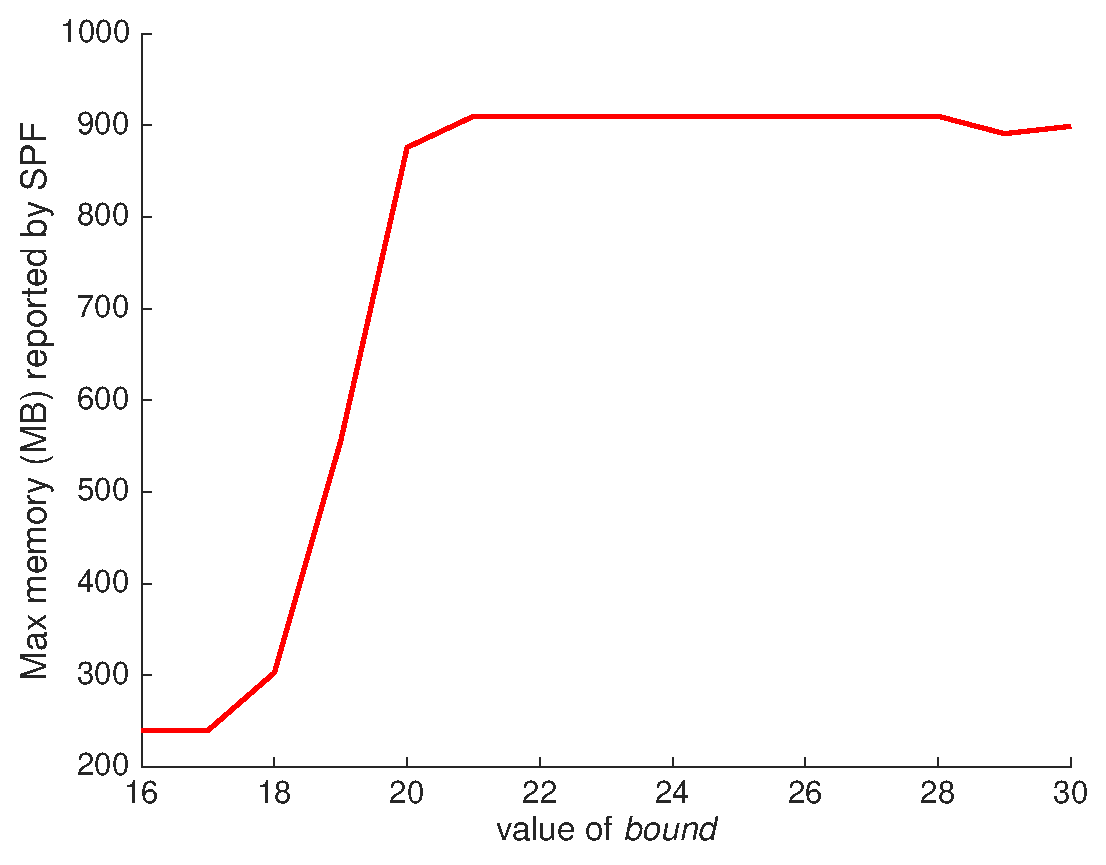
\includegraphics[width=0.4\columnwidth]{figures/sharing_mem} }\label{fig:sharing_mem}}%
    \caption{Time and memory usage of Listing~\ref{lst:sharing} when increasing \textit{bound}}%
    \label{fig:sharing}%
    \vspace{-0.2in}
\end{figure}
%
Figure~\ref{fig:sharing_mem} shows that at a value of 17 for \textit{bound}, the memory usage starts to rise from 240 MB and has reached 910 MB when \textit{bound} equals 21.
%
We also observed that the number of expression objects undergoes a linear increase with the value of \textit{bound}.
%
These three observations lead us to the hypothesis that while SPF does share expression objects internally, the traversal of such expressions breaks the sharing and causes an increase in time and memory.
%
%The time increase is due to garbage collection once the maximum memory threshold is reached.
%
%Integrating veritesting with SPF to make it scale to industrial-sized code requires resolving such engineering issues.
%
\subsection{Complex Expressions}
%Engineering issue \#2: Need to have complex expressions, talk about how Comparators cannot be used anywhere below the top-level operator
During exploration, SPF creates conjunctions of expressions and adds them to its {\em PathCondition} to determine satisfiability of paths.
%
These expressions are allowed to have a \textit{Comparator}~(a comparison operator such as !=) as the top-level operator; however, comparison and Boolean operators are not allowed in sub-expressions.  Thus, the current set of SPF expressions is insufficiently expressive to represent the disjunctive formulas required for multi-path regions.%, and we are currently refactoring the SPF expression hierarchy to allow for richer expression types.
%
%Because SPF has different classes for different expression types~(\textit{IntegerExpressions}, \textit{RealExpression}), these changes must be made in several different places; we believe that moving forward, the
%
%Thus, integrating veritesting presents a design challenge to allow complex expressions in SPF.
%
% \subsection{Intermediate variables}
% %Engineering issue \#3: Nice to introduce intermediate variables
% %
% During veritesting, symbolic formulas derived from static symbolic execution of a region may involve conditional write operations into other variables.
% %
% It is convenient to have intermediate variables~(one per variable written to in the region) which capture such conditional write expressions during the static symbolic execution.
% %
% Later, at an exit point, the intermediate variables can be written into the original variables written to in the region.
% %
% This allows sub-expressions to be shared, and even simplified, without affecting the original variables from the Java bytecode.
% %
% Smaller formulas written into the region\rq s output variables also makes it easier to debug veritesting of regions.
% %
% However, creation of such intermediate variables presents a design challenge in SPF.
% %
% SPF stores and propagates symbolic information through attribute objects.
% %
% This, in turn, creates an invariant that every symbolic variable in the path expression needs to be mapped to an attribute object.

%
%
% \subsection{Veritesting with Multi-threading}
% Veritesting requires SPF to be able to perform static symbolic execution on a region of code and incorporate it as a disjunctive predicate into its path expression along with the corresponding updates to its symbolic store.
% %
% If the region being statically analyzed can be executed in a multi-threaded context, however, then it is necessary to consider all possible points of interference in the region.
% %
% This consideration requires changes to the updates made to SPF\rq s path expression and its symbolic store.
% %
% One way to handle this is to turn every point of interference as an exit point, but determining the possible points of interference statically is itself a difficult problem.  Likely it will require some level of dynamic analysis to determine the points of interference at the time of creation of a veritesting region.
% %
% %But, veritesting would be beneficial if its static analysis also includes computation of points at which interference is infeasible.
% %
% This makes creating an efficient veritesting approach challenging since the cost of this computation must be less than the cost of doing plain dynamic symbolic execution.
















% Data from perl script-based static analysis
% this script just counted the difference between instructions
%
% \begin{table}[]
% \centering
% \caption{My caption}
% \label{my-label}
% \begin{tabular}{|l|l|l|l|}
% \hline
%         & if-ret & if-IV & if-throw \\ \hline
% Chart   & 8.08   & 5.79  & 6.10     \\ \hline
% Closure & 7.40   & 4.37  & 12.6     \\ \hline
% Lang    & 6.3    & 5.23  & 8.26     \\ \hline
% Math    & 12.9   & 6.9   & 9.09     \\ \hline
% Mockito & 8.5    & 4.38  & 11.39    \\ \hline
% Time    & 9.0    & 5.56  & 9.3      \\ \hline
% \end{tabular}
% \end{table}

\section{Related Work}
%Talk about veritesting in Mayhem, Angr.
%
The original idea for veritesting was presented by Avgerinos et al.~\cite{veritesting}.
%
They implemented veritesting on top of MAYHEM~\cite{mayhem}, a system for finding bugs at the X86 binary level which uses symbolic execution.
%
Their implementation demonstrated dramatic performance improvements and allowed them to find more bugs, and have better node and path coverage.
%
Veritesting has also been integrated with another binary level symbolic execution engine named {\tt angr}~\cite{angr}.
%
Veritesting was added to {\tt angr} with similar goals of statically and selectively merging paths to mitigate path explosion.
%
However, path merging from veritesting integration with {\tt angr} caused complex expressions to be introduced which overloaded the constraint solver.
%
Using the Green~\cite{green} solver may alleviate such problems when implementing veritesting with SPF.
%
Another technique named \textit{MultiSE} for merging symbolic execution states incrementally
was proposed by Sen et al.~\cite{multise}.
%
MultiSE computes a set of guarded symbolic expressions for every
assignment and does not require identification of points where
previously forked dynamic symbolic executors need to be merged.
%
MultiSE complements predicate construction for multi-path regions beyond
standard exit points~(such as
\textit{invokevirtual},~\textit{invokeinterface},~\textit{return}
statements).
%
Combining both techniques, while a substantial implementation effort, has the potential
to amplify the benefits from both techniques.
%This observation became even more apparent for longer paths.
%
%Integrating veritesting with SPF may expose a similar trade-off.
%
%But we expect this problem to be less severe for when doing static symbolic execution of Java bytecode because Java bytecode instructions have fewer behaviors to be statically analyzed than X86 architecture instructions.

% %Talk about other symbolic execution performance improvements.
% %mentioned in Christopher Kruegel's ISSTA keynote talk as Static Analysis support
% Other static analysis techniques also provide support for dynamic symbolic execution.
% %
% Loop-extended symbolic execution introduced partial loop summarization by having symbolic variables that represent the number of times each loop executes.
% %
% This technique allowed symbolic variables to incorporate loop dependent effects along with data dependencies from program inputs.
%
%Value Set Analysis~\cite{vsa} is another static analysis technique that can potentially benefit dynamic symbolic execution.
%%
%Value set analysis uses an abstract domain to find an over-approximated set of values that registers or abstract locations may have at program points.
%%
%Value set analysis can help dynamic symbolic execution resolve ranges without solving constraints.
%VSA can resolve ranges without solving constraints, thereby, finding applications in computing all possible write targets during a memory write operation.
%Code summarization (Dodo)
%  - automatically (and statically) summarize effect of loops / functions
%VSA - value set analysis
%  - resolve ranges (and conditionals) without solving constraints

%Talk about TamiFlex, and how using the same technique as TamiFlex is one way to solve veritesting challenges in Java bytecode.
%
%Other techniques for static analysis at the Java bytecode level can also benefit dynamic symbolic execution.
%
Finding which reflective method call is being used, or handling dynamic class loading are known problems for static analysis tools.
%
TamiFlex~\cite{tamiflex} provides an answer that is sound with respect to a set of previously seen program runs.
%
Integrating veritesting runs into similar problems, and using techniques from TamiFlex would allow static predicate construction beyond exit points caused by reflection or dynamic class loading. 

\section{Technique}
%
To add path merging to SPF, we first pre-compute static summaries of arbitrary code regions with more than one execution
path and we also pre-compute method summaries.
%
To bound the set of code regions we analyze, we start by specifying a method $M$ in a configuration file.
%
Next, we construct a set containing only the class $C$ that contains $M$.
%
We then get another set of classes, $C'$,
such that every class in $C'$ has at least one method that was called by a method in a class in $C$.
%
This step which goes from $C$ to $C'$ discovers all the classes at a call depth of 1 from $C$.
%
We continue this method discovery process up to a call depth of 2.
%
While we can increase the call depth in our method discovery process, we found that summarizing
arbitrary code regions with more than 2 calls deep, did not lead to practically useful region summaries.
%
After obtaining a list of methods, we computed static summaries of regions in these methods and method summaries as
explained in Section \ref{sec:static-analysis}.
%
After computing static region and method summaries, we process them as a sequence of transformations described in the next section~\ref{sec:instantiationTransformations} and summarized
in Figure~\ref{fig:overview}.
%
\begin{figure}[]
    \caption{Overview of transformations on Ranger IR to create and instantiate multi-path region summaries with higher-order regions}
    \label{fig:overview}
    \includegraphics[width=\textwidth]{figures/overview.pdf}
\end{figure}
%
%
%\subsection{WALA-based analysis for veritesting}
%%
%Veritesting requires static construction of
%predicates of a multi-path region which represent changes to the path expression of the dynamic
%symbolic executor.
%%
%It also requires construction of a control-flow graph of method bodies
%from Java bytecode and finding exit points of the region, which in turn
%requires creation of a control-flow graph of the region.
%%
%Implementing veritesting is made simpler by using a static single
%assignment~(SSA)~\cite{ssa} representation of the multi-path region.
%%
%Using an SSA form allows us to use the $\phi$-expressions created by the
%SSA form and translate them into points at the end of the veritesting
%region where updates to system state along different paths in the region
%can be merged.
%%
%\mike{MWW: Vaibhav please update to describe WALA}
%WALA~\cite{} is a static analysis framework for Java programs that
%has both these features, with
%ExceptionalUnitGraph~\cite{exceptionalunitgraph} and the Shimple
%IR~\cite{shimple}.
%%
%For simple regions with only one exit point, like the one presented in Listing~\ref{lst:v_ex}, we
%were able to use Soot to automate static construction of the predicate representing
%an update to the expression.
%%
%For doing this, we used nodes with more than one successor as the
%starting point, found the immediate post-dominator of the starting
%point, and traversed the control-flow graph on all sides of such branches.
%%
%During such a traversal, we constructed predicates representing the
%multi-path region, similar to the ones presented in
%Listing~\ref{lst:v_ex_smt2}.
%%
%As explained in Section~\ref{sec:exit_points}, including virtual
%function invocations in the construction of our predicates amplifies the
%benefits of veritesting even further.
%%
%We plan to automate this inclusion in the future using Soot.
%%
%Providing SPF with updates to be made to its symbolic store also
%requires Soot to maintain stack location information for variables.
%%
%We plan to automate SPF\rq s symbolic store updates using Soot in the
%future.
%%
%

\subsection{Statement Recovery}
\label{sec:static-analysis}
%Java Ranger has its own AST that captures the statement of regions.
%%
%The choice of having a separate AST for Java Ranger, enables the integration of Java Ranger with any static analysis framework by implementing the transformation that transforms the CFG of a given IR into the corresponding Java Ranger AST representation. 
%%
%We call this interface \textit{Statement Recovery} transformation. \\
%%
%In this transformation we visit nodes in topological order by walking normal edges of a branching points until a \textit{minimum convergent node} is encountered. We define a minimum convergent node as the last immediate successor of blocks following a branching node.
%%
%Note that exceptional edges are ignored during this transformation, however exceptional behavior is later identified and handled through the single path cases.
%%
%We discuss more about this in section~\ref{sec:instantiationTransformations}.
%%
%There are two other things that this transformation takes care of: recovering of complex if-then-else and construction of Gated Single Assignment (GSA).
%%
%Recovering of complex conditions in an if-statement restores its form in the source code. 
%% 
%This is done by identifying \textit{immediate self-contained subgraphs}, that is, subgraphs where the initial node is immediately pre-dominated by the initial node and for the static region and whose successor nodes (up to the region terminus) are dominated (not necessarily immediately) by the initial node.
%%
%
%Construction of Gated Single Assignment (GSA) on the other hand is done by keeping track of the current "conditional path" during translation. More precisely this is done by keeping a stack of  {\tt(Expression x enum \{Then, Else\})} pairs. 
%%
%In addition to that, for each edge between blocks in the block structure, the associated "conditional path" is recorded.  
%%
%So the type of this map (the blockConditionMap) is: {\tt(ISSABasicBlock x ISSABasicBlock) --> List of (Expression x enum \{Then, Else\})}.
%%
%Finally creation of the condition of GSA is done during translating a phi-instruction its immediate predecessor blocks are retrieved then we look up  the edges in the blockConditionMap.  From here, and using condition stack leading to that branch, an if/then/else statement is constructed.

The regions of interest for our technique are bounded by the branch and meet of a given acyclic subgraph.  The intuition is that path explosion during execution of loops is driven by conditional logic within the loop, rather than the loop itself.
Starting from an SSA form, the first transformation recovers a tree-shaped AST for the subgraphs of interest.  While this step is not strictly necessary, it substantially simplifies subsequent transformations.  

The algorithms are similar to those used for those used for decompilation~\cite{Yakdan15@decompilation} but with slightly different goals: 
\begin{itemize}
    \item The algorithm must be {\em accurate} but need not be {\em complete}.  That is, obfuscated regions of code need not be translated into a tree form.
    \item The algorithm must be {\em lightweight} in order to be efficiently performed during analysis.  Thus, algorithms that use global fixpoint computations are 
        too expensive to be used for our purposes.
\end{itemize}

Starting from an initial SSA node, the algorithm first finds the immediate post-dominator of all {\em normal} control paths, that is, paths that do not end in an exception or return instruction.  It then looks for nested self-contained subgraphs.  If for any graph, the post-dominator is also a predecessor of the node, we consider it a loop and discard the region.  

The algorithm systematically attempts to build regions for every branch instruction, even if the branch is already contained within another region.  The reason is that it may not be possible to instantiate the larger region depending on whether summaries can be found for {\em dynamically-dispatched} functions, and whether references are {\em uniquely determinable} for region outputs.

\iffalse
\begin{verbatim}

stmt ::= stmt ; 
   

\end{verbatim}

\vaibhav{assigned to Mike}
\mike{MWW: - we should provide an AST of the constraint language}
\fi 

\subsection{Region Definition}

Once the statement of a multi-path region has been recovered, its corresponding environment is populated.
%
This includes identifying region boundary and creating local variable inputs, outputs, type, and stack slot tables for
the region.
%
The region boundary is used to identify boundaries of the region w.r.t local variables.
%
This is used later to constrain the computation and population of Ranger IR environment tables.
%
For example, the local variable input table is populated with first \textit{use} in the region boundary that map to a given stack slot.
%
The output table is populated with the last \textit{def} of a local variable at merge point of the region.
%
The local variable type table is populated for all variables that lay within the boundaries of the region, this is initially done by
inquiring the static analysis framework, WALA~\cite{Wala} but is later changed by inferring types of local variables
at instantiation and during type propagation transformation~\ref{sec:instantiationTransformations}.

We also construct a stack slot table as part of a region\rq s Ranger IR summary.
%
The stack slot table maps Ranger IR variables to a stack slot, if they correspond to a local variable in the source code.
%
We populate the stack slot table by obtaining a variable to stack slot mapping from WALA.
%
We also assume that, if at least one variable used in a $\phi$-expression is a local variable, then all variables
used in that $\phi$-expression must belong to the same stack slot.
%
We use this assumption to further propagate stack slot information in the stack slot table across all $\phi$-expressions
encountered at merge points of regions.

%The stack slot table on the other hand, does not use region boundary for its population. The reason for this is that,
%the static analysis framework we use, WALA, sometime does not provide information about the stack slots of intermediate
%variables.
%%
%This is particularly problematic in our case because the def of a phi is both an intermediate variable, and so we do
%not know its stack slot, yet it is also an output of the region for which we want to populate its symbolic
%representation onto the stack slot.
%%
%Therefore, our stack slot table uses stack slot inference by propagating the stack slots of vars used in a phi onto the
%def of the phi.
%%
%This requires visiting all variables and phi statements of the IR to maximize the inference of the stack slot, this is
%repeatedly done until a fix point is reached.


\subsection{Instantiation-time Transformations}
\label{sec:instantiationTransformations}

\textbf{Renaming Transformation}: In Alpha renaming transformation, all Ranger IR variables are renamed to ensure their uniqueness before further processing takes place. 
%
This is particularly important not only to ensure uniqueness of variables among different regions, but also to ensure
uniqueness of variable names of the \textit{same} region which might be instantiated multiple times on the same path,
i.e., a region inside a loop will be instantiated multiple times.\\
%
\textbf{Local Variable Substitution Transformation}: During this transformation we eagerly bring in all dynamically
known constant values, symbolic values and references from stack slots into the region for further processing. \\
%
\textbf{Higher-order Regions Transformation}: This transformation is initiated when a method invocation is encountered
during local variable substitution.
%
At this point, we perform three steps.
%
(1) the region that corresponds to the called method is retrieved and alpha renaming of
Ranger IR variables corresponding to local variables is applied on it.
%
(2) Ranger IR expressions that correspond to the actual parameters are evaluated and used to substitute the formal
parameters by repeatedly applying local variable substitution transformation over the method region.
%
(3) When no more higher-order regions can be inlined, the resulting substituted method region is inlined into
the outer region.\\
%
If the method region has a single return value, then the original method invocation is replaced with an assignment to
the returned expression.
%
%Otherwise, inlining of the method region takes place.
%
We dont currently support instantiation of method regions with multiple return statements, support for which requires
another transformation that we talk about in Section~\ref{sec:future}.
\\
\textbf{Field References SSA form}: The field references transformation translates reads and writes of fields
in Java bytecode into corresponding Ranger IR statements.
%
In order to translate all field accesses to SSA form, this transformation creates a summary of the semantics
represented by the field accesses in the region.
%
This transformation constructs a new field access variable for every field assignment on every path within the region.
%
This new field access variable construction makes use of two monotonically increasing subscripts.
%
It uses a path subscript to distinguish between assignments to the same field on the same execution path.
%
It uses a global subscript to distinguish between assignments to the same field across execution paths.
%
At the merge point of the region, field assignments done on the same field are merged using
Gated Single Assignment (GSA)~\cite{Ottenstein1990}.
%
Each merged field access variable has its own path and global subscripts and represents the output of the region into
its field.
%
The path subscript helps us resolve read-after-write operations on the same execution path and find the latest write
into a field on an execution path.
%
The global subscript helps us distinguish between field accesses across multiple execution paths. \\
\textbf{Array References SSA form}: The array references transformation translates reads and writes of arrays in
Java bytecode into corresponding Ranger IR statements.
%
In order to translate all array accesses to SSA form, this transformation creates an execution path-specific copy of
every array when it is first accessed within a region.
%
Reads and writes of arrays are then done on a path-specific copy of the array.
%
All array copies are merged at the merge point of multi-path regions.
%
The merged array copy represents array outputs of the region.\\
\textbf{Type Propagation}: Ranger IR needs to have type information for its variables so that it can construct
corresponding correctly-typed Green variables during the final transformation of the region summary to a Green formula.
%
Having accurate type information is also important for looking up the correct higher-order method summary.
%
As part of region instantiation, Java Ranger infers types of Ranger IR variables in the region summary by
using JPF's runtime environment.
%
Types of local variables are inferred during the local variable substitution transformation and types of field reference
and array reference variables are inferred during their respective transformations.
%
Using these inferred types, the type propagation transformation propagates type information across assignment
statements, binary operations, and variables at leaf nodes of $\gamma$ functions.\\
%
\textbf{Simplification of Ranger IR}: The Ranger IR constructed by earlier transformations computes exact semantics
of all possible behaviors in the region.
%
Representation of such semantics as a formula can often lead to unnecessarily large formulas, which has the potential to
reduce the benefits seen from path merging~\cite{angr}.
%
For example, if an entry in an array is never written to inside a region, the array reference transformation can still have an
array output for that entry that writes a new symbolic variable into it.
%
The region summary would then need to have an additional constraint that makes the new symbolic variable equal the
original value in that array entry.
%
Such conjuncts in the region summary can be easily eliminated with constant propagation, copy propagation, and constant
folding~\cite{dragon-book}.
%
Ranger IR also has statement and expression classes that use a predicate for choosing between two statements (similar to
an {\tt if} statement in Java) and two sub-expressions (similar to the C ternary operator) respectively.
%
When both choices are syntactically equal, the predicated statement and expression objects can be substituted with the
statement or expression on one of their two choices.
%
Such statements and expressions were simplified away to use one of their two choices.
%
Ranger IR performs these two simplifications on such predicated statements and expressions along with constant folding,
constant propagation, and copy propagation.\\
\textbf{Single Path Cases}: This transformation collects path predicates inside a region that lead to
\textit{non-nominal} exit point.
%
This is an alternative approach to that was presented in \cite{veritesting}.
%
In our work we define non-nominal exit point to be points inside the region that either define exceptional behavior or
involve behavior that we cannot summarize, i.e, object creation and throw instructions.
%
The intuition here is that, we want to maximize regions that Java Ranger can summarize, even if the summarization is
only partial.
%
We use this pass of transformation to identify such points, collect their path predicates and prune them away from the
Ranger IR statement.
%
The outcome of this process, is a more simplified and concise statement that represent the nominal behavior of the Ranger region.
%
The collected predicate is later used to guide the symbolic execution to explore non-nominal paths, which Java Ranger
had not summarized.  \\
%
\textbf{Linearization}:
Ranger IR contains translation of branches in the Java bytecode to if-then-else statements defined in the Ranger IR.
%
But the if-then-else statement structure needs to be kept only as long as we have more GSA expressions to be
introduced in the Ranger IR.
%
Once all GSA expressions have been computed, the Ranger IR need not have if-then-else statements anymore.
%
The $\gamma$ functions introduced by GSA are a functional representation of branching, which lets us
capture the semantics of everything happening on both sides of the branch.
%
Since the linearization transformation is done after every field and array entry has been unaliased and converted to
GSA, dropping if-then-else statements from the Ranger IR representation of the region summary reduces redundancy in its
semantics and converts it into a stream of GSA and SSA statements.\\
\textbf{Translation to Green}:
%
At this point Ranger region contains only compositional statements as well as assignment statements that might contain GSA expressions in them.
%
This transformation starts off by translating Ranger variables to Green variables of the right type using the region type table.
%
Then Ranger statements are translated. More precisely, compositional statements are translated into conjunction, assignment statements are translated into Green equality expressions.
%
For assignment statements that have GSA expressions, these are translated into two disjunctive formulas that describes the assignment if the GSA condition or its negation were satisfied. 

\subsection{Checking Correctness Of Region Summaries}
The Ranger IR computed as a result of performing the transformations described in Figure~\ref{fig:overview} should
correctly represent the semantics of the summarized region.
%
If it does not, then using the instantiated region summary can cause symbolic exploration to explore the wrong behavior
of the subject program.
%
We checked the correctness of our instantiated region summaries by using equivalence-checking as defined by Ramos et al.~\cite{ramos}.
%
We designed a test harness that first executes the subject program with a set of symbolic inputs using SPF and
capture the outputs of the subject program.
%
Next, the test harness executes the same subject program with the same set of symbolic inputs using Java Ranger and
capture the outputs of the subject program once again.
%
Finally, the test harness compares outputs returned by symbolic execution with SPF and Java Ranger.
%
If the outputs do not match, then a region summary used by Java Ranger did not contain all the semantics
of the region it summarized.
%
We symbolically execute all execution paths through this test harness.
%
If no mismatch is found between outputs on any execution path, we conclude that all region summaries used by Java Ranger
must correctly represent the semantics of the regions they summarized.
%
We performed correctness-checking on all results reported in this paper.

%\section{Experiment}
\vaibhav{assigned to Vaibhav}

We would like to measure the performance of \tool\ against the baseline of single-path exploration using Java Symbolic
PathFinder.  This can be examined in several dimensions: the wall-clock time of the solving process, the number of paths
explored.  In addition, we would also like to gather metrics about the regions themselves, in order to better understand
where static regions are effective.

Therefore, we investigate the following research questions:

\begin{description}
\item[RQ1:] How much do higher-order static regions (HOSR) improve the performance of symbolic execution?
\item[RQ2:] How much do HOSRs reduce the number of paths explored?
\item[RQ3:] How do HOSRs affect the number and expense of calls to the SMT solver?
\item[RQ4:] How does the size of computed HOSRs affect the performance of the approach?
\end{description}

For each question, we examine three different configurations of \tool: a version that creates simple regions (one
branch) only (\tool-SR), one that creates complex regions with multiple branches but no non-local jumps (\tool-CR), and
one that operates over higher-order complex regions containing non-local jumps (\tool-CR+HO). This allows us to examine
(at a coarse level) how each feature impacts the experimental results.

\subsection{Experimental Setup}

\mike{Information here about benchmark models and machine configuration}

\mike{The benchmarks should be a superset of at least one previous paper, and better yet, multiple papers}. 
\section{Evaluation}
\label{sec:results}
\subsection{Experimental Setup}
%
We implemented the above mentioned transformations as a wrapper around the Symbolic PathFinder~\cite{spf} tool.
%
To make use of region summaries in Symbolic PathFinder, we use an existing feature of SPF named \textit{listener}.
%
A listener is a method defined within SPF that is called for every bytecode instruction executed by SPF.
%
\tool\ adds a path merging listener to SPF that, on every program location to be executed, checks if the next
instruction is a conditional branch instruction with at least one symbolic operand.
%
On finding such a symbolic branch condition, \tool\ attempts to compute a static summary of all multi-path
regions in the method which contains the current program location.
%
After this Just-In-Time static analysis, if \tool\ summarized the multi-path region that begins at the current program
location, \tool\ instantiates the region summary corresponding to the current program location by reading inputs from
and writing outputs to the stack and the heap.
%
Finally, it conjuncts the instantiated region summary with the path condition and resumes symbolic execution at the
bytecode offset of the end of the region.
%
\tool\ wraps around SPF and can be configured to either run SPF without any path merging or run SPF with the
following path-merging features enabled.

\tool\ summarizes multi-path regions with a single exit point and instantiates them if they are encountered.
This includes multi-path regions that have local, stack, field, or array outputs.
%
\tool\ substitutes local inputs into the Ranger IR representation of the multi-path region, and constructs SSA form
Ranger IR for all field and array accesses in the region using its instantiation-time context.
%
The SSA form representation of all field and array accesses allows the Ranger IR to be simplified uniformly across all
variable types which reduces the size of the region summary and improves performance.
%
While our current implementation of \tool\ cannot instantiate summaries with symbolic object and array
references, it is capable of summarizing reads and writes to arrays with symbolic indices.
%
\tool\ instantiates all multi-path region
summaries that make method calls which have also been statically summarized.
%
Method summaries are inlined into
the multi-path region summary based on the instantiation-time type of the method.
%
\tool\ uses single-path cases to allow regions to have more than one exit point.
%
These exit points take the form of new object allocations and exceptional behavior present in the region.
%
\tool\ converts multiple exit points that return
control flow from the region to its caller into a single control flow-returning exit point.
%
This feature allows summarization of multiple {\tt return} instructions in a region into a single control-flow
returning exit point.
%
Instead of a single return value, such an exit point returns a formula to its caller, which predicates
each return value on its corresponding condition in the region.

We used the control-flow graph recovered by Wala~\cite{Wala} to bootstrap our static statement recovery process.
%
%While we found our static statement recovery was capable of summarizing thousands of regions in Java library code, many
%of these summaries could not be instantiated due to JPF\rq s use of native peers~\cite{jpf-mji}.
%
%To avoid these unnecessary instantiation failures and target our static statement recovery towards the benchmark code,
%we turned off statement recovery across a few Java library packages in Wala on all benchmarks.
%
We ran the above implementation using the incremental solving mode of Z3 using the bitvector theory.
%
The incremental solving mode provides only the last constructed constraint to the solver instead of passing the entire
path condition every time a query is to be solved.
%
Since path-merging can create large formulas in the path condition, the incremental solving mode provided a crucial
benefit in reducing the number of times large formulas had to be passed to the solver.
%
\subsection{Evaluation}
%
In order to evaluate the performance of \tool, we used the following nine benchmarking programs commonly used to
evaluate symbolic execution performance.
%
Eight of these programs were provided by Wang et al.~\cite{dgse} which also includes a translation of the
Siemens suite to Java.
%
(1) Wheel Brake System (WBS)~\cite{yang2014directed} is a synchronous reactive
component developed to make aircraft brake safely when taxing, landing, and during a rejected take-off.
%
(2) Traffic Collision Avoidance System (TCAS) is part of a suite of programs commonly referred to as the Siemens
suite~\cite{siemens-benchmarks}. TCAS is a system that maintains altitude separation between aircraft to avoid mid-air
collisions.
%
(3) Replace is another program that\rq s part of the Siemens suite. Replace searches for a pattern in a given input and
replaces it with another input string.
%
(4) NanoXML is an XML Parser written in Java which consists of 129 procedures and 4608 lines of code.
%
(5) Siena~(Scalable Internet Event Notification Architecture) is an Internet-scale event notification middleware for
distributed event-based applications~\cite{siena} which consists of 94 procedures and 1256 lines of code.
%
(6) Schedule2 is a priority scheduler which consists of 27 procedures and 306 lines of code.
%
(7) PrintTokens2 is a lexical analyzer which consists of 30 procedures and 570 lines of code.
%
(8) ApacheCLI~\cite{apachecli} provides an API for parsing command lines options passed to programs.
It consists of 183 procedures and 3612 lines of code.
%
(9) MerArbiter models a flight software component of NASA JPL\rq s Mars Exploration Rovers.
%
%It was originally modeled in Simulink/Stateflow and automatically translated into Java using the Polyglot framework.
%
We used the version made
available by Yang et al.~\cite{memoise}. This benchmark consists of 268 classes, 553 methods, 4697 lines of code
including the Polyglot framework.

We first ran each of these benchmarks using SPF with increasing number of symbolic inputs and obtained the most number of inputs
with which SPF finished complete exploration of each benchmark within a 24 hour time budget.
%
We then ran each benchmark with this number of symbolic inputs with \tool.
%
This evaluation allowed us to check if \tool\ is faster than SPF at achieving complete path exploration of each benchmark.
%
Next, we used the fastest mode of \tool\ to check if it could explore the benchmark with even more symbolic inputs within
the same 12 hour time budget.\vaibhav{Figure out if these results need to be reported}
%
We report results from this evaluations for each benchmark in Table~\ref{table:results-all-mode5}
%
Since Java Ranger relies on a prior static analysis to construct region summaries, we report the time taken to statically
analyze all the code in each of the benchmarks in column ``static analysis time (sec)'' in
Table~\ref{table:results-all-mode5}.
%
We found that the total time required for static analyis is roughly proportional to the size of the benchmark.
%
While static analysis performance can cause \tool\ to be slower on benchmarks with a small number of execution
paths, we observed that the cost of static analysis gets amortized as the number of execution paths increases.
%
% Please add the following required packages to your document preamble:
% \usepackage{booktabs}
\begin{table*}[]
    \centering
    \caption{Comparing the performance of \tool\ with Symbolic PathFinder on 9 benchmarks. ``\# sym inputs` indicates the
    total number of symbolic inputs that were given to each benchmark. For WBS and TCAS, we ran WBS and TCAS with
    path-merging using symbolic inputs corresponding to 10 steps of each.
    ``path-merging enabled'' indicates a comparison of no path-merging with path-merging with
    all the features turned on.}
    \label{table:results-all-mode5}
    \begin{tabular}{@{}ccccccccccc@{}}
        \toprule
        \begin{tabular}[c]{@{}c@{}}Benchmark\\ name\end{tabular} & \begin{tabular}[c]{@{}c@{}}\#\\ sym\\ inputs\end{tabular} & \begin{tabular}[c]{@{}c@{}}path-\\ merging\\ enabled?\end{tabular} & \begin{tabular}[c]{@{}c@{}}total\\ runtime\\ (sec)\end{tabular} & \begin{tabular}[c]{@{}c@{}}static\\ analysis\\ time\\ (sec)\end{tabular} & \begin{tabular}[c]{@{}c@{}}\#\\ exec.\\ paths\end{tabular} & \begin{tabular}[c]{@{}c@{}}\#\\ solver\\ queries\end{tabular} & \begin{tabular}[c]{@{}c@{}}solver\\ time\\ (sec)\end{tabular} & \begin{tabular}[c]{@{}c@{}}\# distinct\\ regions\\ used\end{tabular} & \begin{tabular}[c]{@{}c@{}}\# inlined\\ method\\ summaries\end{tabular} & \begin{tabular}[c]{@{}c@{}}\# fully-linearized\\ region\\ summaries\end{tabular} \\ \midrule
        WBS                                                      & 15                                                        & NO                                                                 & 4427.66                                                         & 0                                                                        & 7962624                                                    & 15925246                                                      & 3121.44                                                       & 0                                                           & 0                                                                    & 0                                                                    \\
        WBS                                                      & 30                                                        & YES                                                                & 2.81                                                            & 3.73                                                                     & 1                                                          & 0                                                             & 0                                                             & 16                                                          & 0                                                                    & 140                                                                  \\ \midrule
        TCAS                                                     & 24                                                        & NO                                                                 & 353.07                                                          & 0                                                                        & 39204                                                      & 465262                                                        & 296.23                                                        & 0                                                           & 0                                                                    & 0                                                                    \\
        TCAS                                                     & 120                                                       & YES                                                                & 1.41                                                            & 2.29                                                                     & 1                                                          & 0                                                             & 0                                                             & 4                                                           & 560                                                                  & 40                                                                   \\ \midrule
        replace                                                  & 11                                                        & NO                                                                 & 1176.83                                                         & 0                                                                        & 757261                                                     & 4317642                                                       & 749.77                                                        & 0                                                           & 0                                                                    & 0                                                                    \\
        replace                                                  & 11                                                        & YES                                                                & 4581.13                                                         & 7.97                                                                     & 91983                                                      & 1441674                                                       & 3563.57                                                       & 20                                                          & 360                                                                  & 7334                                                                 \\ \midrule
        NanoXML                                                  & 8                                                         & NO                                                                 & 63554.90                                                        & 0                                                                        & 33944190                                                   & 77831662                                                      & 30071.39                                                      & 0                                                           & 0                                                                    & 0                                                                    \\
        NanoXML                                                  & 8                                                         & YES                                                                & 28803.23                                                        & 13.31                                                                    & 3637075                                                    & 10363980                                                      & 19742.50                                                      & 10                                                          & 8136                                                                 & 990022                                                               \\ \midrule
        Siena                                                    & 7                                                         & NO                                                                 & 55027.94                                                        & 0                                                                        & 35831808                                                   & 91208236                                                      & 26689.72                                                      & 0                                                           & 0                                                                    & 0                                                                    \\
        Siena                                                    & 7                                                         & YES                                                                & 57782.26                                                        & 23.66                                                                    & 35831808                                                   & 91208236                                                      & 26945.8                                                       & 0                                                           & 0                                                                    & 0                                                                    \\ \midrule
        Schedule2                                                & 3                                                         & NO                                                                 & 1.48                                                            & 0                                                                        & 343                                                        & 684                                                           & 0.33                                                          & 0                                                           & 0                                                                    & 0                                                                    \\
        Schedule2                                                & 3                                                         & YES                                                                & 2.52                                                            & 3.42                                                                     & 343                                                        & 684                                                           & 0.32                                                          & 0                                                           & 0                                                                    & 0                                                                    \\ \midrule
        PrintTokens2                                             & 4                                                         & NO                                                                 & 1716.27                                                         & 0                                                                        & 166644                                                     & 3491916                                                       & 1305.59                                                       & 0                                                           & 0                                                                    & 0                                                                    \\
        PrintTokens2                                             & 4                                                         & YES                                                                & 1338.85                                                         & 4.01                                                                     & 109727                                                     & 2404854                                                       & 634.34                                                        & 4                                                           & 0                                                                    & 122504                                                               \\ \midrule
        ApacheCLI                                                & 6+1                                                       & NO                                                                 & 31886.46                                                        & 0                                                                        & 4839812                                                    & 64432586                                                      & 9470.83                                                       & 0                                                           & 0                                                                    & 0                                                                    \\
        ApacheCLI                                                & 6+1                                                       & YES                                                                & 5560.94                                                         & 10.12                                                                    & 171818                                                     & 756030                                                        & 1904.21                                                       & 5                                                           & 0                                                                    & 977972                                                               \\ \midrule
        MerArbiter                                               & 28                                                        & NO                                                                 & 70876.22                                                        & 0                                                                        & 2429568                                                    & 6816406                                                       & 3391.12                                                       & 0                                                           & 0                                                                    & 0                                                                    \\
        MerArbiter                                               & 28                                                        & YES                                                                & 11087.11                                                        & 5.96                                                                     & 276144                                                     & 910023                                                        & 475.49                                                        & 16                                                          & 0                                                                    & 411227                                                               \\ \bottomrule
    \end{tabular}
\end{table*}
%
Table~\ref{table:results-all-modes5} shows that \tool\ achieves a significant speed-up over SPF with
5~(WBS, TCAS, NanoXML, ApacheCLI, MerArbiter) of the 9 benchmarks in terms of both running time and number of
execution paths.
%
Of the remaining four benchmarks, \tool\ also achieves a modest 22\% reduction in running time and 34\% reduction
in the number of execution paths with the PrintTokens2 benchmark.
%
\tool\ has the same performance as SPF on Siena and Schedule2 with a minor overhead in running time that comes from
\tool\rq s lookup of a region summary for every executed branch instruction and recording of instantiation-time metrics.
%
We restrict our results with Siena to 7 symbolic inputs because 6 is the most number of symbolic inputs for which
SPF finishes complete path exploration within a 24 hour time budget.
%
On running Siena, the overhead of \tool\ results from running into concrete branch instructions that
\tool\ could have summarized, had these branches been symbolic.
%
In the replace benchmark, while \tool\ reduces the number of execution paths by about 89\%, it incurs an increase in
execution time due to most region instantiations not being beneficial.
%
On manually investigating the set of instantiated regions in replace, we found that the outputs of most regions were
being branched on later in the code causing the benefit from more instantiations to be lost.
%
\vaibhav{Running an automated analysis to check if there is a subset of regions that is most beneficial}

\tool\ is able to summarize the entire step function of WBS and TCAS into a single execution path.
%
In case of WBS, \tool\ summarizes a multi-path region that consists of 9 branches.
%
In case of TCAS, \tool\ uses 28 method summaries in each step of TCAS, many of which summarize multiple return values
into a single formula that represents all the feasible return values of the method.
%
While SPF does not finish more than 5 steps of WBS and 2 steps of TCAS within 12 hours, \tool\ finishes 10 steps of both
benchmarks within 59 seconds and 5.6 seconds respectively.

On the NanoXML benchmark, \tool\ finds several opportunities for execution path count reduction on account of the
NanoXML benchmark having several methods with multi-path regions that have a control-flow returning instruction on every
branch side.
%
With mode 5 of \tool\ converting such multiple control-flow returning exit points regions into a single control-flow
returning exit point, \tool\ is able to use more than 27,000 method summaries when running NanoXML with 8 symbolic
inputs and finish in 7.3 hours while vanilla SPF~(which is the same as mode 1 of \tool)
times out in 12 hours.

On the ApacheCLI benchmark, the most significant benefit is introduced in mode 2 of \tool.
%
Modes 4, 5 cause an increase in execution path count and running time but still give a significant reduction over
mode 1.
%
The increase in running time in modes 4 and 5 results from \tool\rq s use of the solver to check if the single-path cases
in modes 4 and 5 are feasible.
%
In the future, we plan to use a counter-example cache to reduce the use of a solver to check the feasibility of these
single-path cases.

In the MerArbiter benchmark, while the most significant benefit is introduced in mode 2 of \tool, the benefit in terms of
both execution path count and running time remains the same in modes 3, 4, and 5.
%
All the multi-path regions that SPF~(which is mode 1 in \tool) needs to branch on but are summarized by \tool\ are small
regions that compute a boolean value based on a symbolic branch and write it to the stack as an operand to be used
by the following return instruction.
%
Most of these multi-path regions lie inside several levels of nested classes and field references that necessitate
a fixed-point computation over the field substitution and constant propagation transformations.
%
\tool\ summarizes such multi-path regions and does 464,000 instantiations with 7 steps of MerArbiter, with more than
319,000 instantiations needing more than 8 iterations of the fixed-point computation.
\section{Future Work}
\label{sec:futureWork}
While \tool\ was able to significantly outperform SPF in a majority of our benchmarks, there are a few directions
along which it can further be extended.
%
Java Ranger attempts to perform path merging as aggressively as possible.
%
This path merging strategy doesn't optimize towards making fewer solver calls.
%
We plan to work towards implementing heuristics that can measure the effect of path merging on the rest of the program.
%
\tool\ currently lacks support for symbolic object and array references.
%
Supporting these would require integrating our implementation with
SPF\rq s lazy initialization~\cite{spf} to allow symbolic object references to be part of a region.

While path-merging gives dynamic symbolic execution a performance boost to explore more paths
efficiently, generating test cases that cover all branches is one of the most useful applications of dynamic
symbolic execution.
%
This is an example of an application of symbolic execution that, if applied as-is, would have to undo the benefits of
path-merging.
%
We intend to extend \tool\ towards test generation for merged paths in the future by targeting test generation
towards a coverage criterion such as Modified Condition/Decision Coverage.

While path merging can potentially allow symbolic execution to explore interesting parts of a program sooner, the
effect of path merging on search strategies, such as depth-first search and breadth-first search commonly used with
symbolic execution, remains to be investigated.
%
We plan to explore the integration of such guidance heuristics with path merging in the future.
%
Java Ranger can summarize methods and regions in Java standard libraries.
%
This creates potential for automatically constructing summaries of standard libraries so that symbolic execution
can prevent path explosion originating from standard libraries.
\section{Conclusion and Future Work}
\label{sec:future}

\soha{we need something for the conclusion}
There are five main directions for future work we intend to do:
\begin{itemize}
\item Support Multiple Return Regions:  Here we want to support regions with multiple returns. 
%
We want to do this by supporting another transformation that would take a multiple return region and turns it into a single return region. 

\item Support of Test Case Generation: while statically summarizing regions gives dynamic symbolic execution a performance boost to explore more paths efficiently, generating test cases that covers all summarized branches is one of the fundamental roles of dynamic symbolic execution that is currently unsupported. 
%
This is one of the extension that we intend to investigate in our future work. 
%

\item Heuristics for Instantiation: as shown in the experiments section, instantiating regions might not always be the best option in terms of performance.
%
For instance, region instantiation could in fact turn concrete values into symbolic values thus increasing the number of explored paths. 
%
This is particularly problematic if that happened for a small region on an early branch point, and the symbolic variable is later used in multiple conditions.
%
This calls for a study of the best heuristics that would provide a decision procedure as to when instantiation a region.

\item Using Incremental Solver: this seems intuitive for two main reasons: firstly because as we go down one path the query sent to the solver is incrementally defined for every branch and yet it is repeatedly being sent to the solver. 
%
And secondly because using Java Ranger tend to have relatively complex formulas to solve due to summarization. 
%
Supporting incremental solver is one direction for our future work. 
\end{itemize}



Other improvements:
\begin{enumerate}
\item Simplification of the Symbolic PathFinder constraint mechanism

\item Interpolation-based path subsumption checks  (c.f.: "More Effective Interpolations in Software Model Checking" - ASE 2017")

\end{enumerate}




\bibliographystyle{splncs04}
\bibliography{references}

\end{document}
